%------------------------------------------------
\begin{frame}
\frametitle{Définitions - cryptage, crypter, chiffrement ?}

\begin{block}{Le chiffrement}
\justifying{
Le chiffrement consiste à chiffrer un document/un fichier à l’aide d’une clef de chiffrement. 
L’opération inverse étant le déchiffrement. 
}
\end{block}
\begin{block}{Le cryptage}
\justifying{
Le terme « cryptage » est un anglicisme, tiré de l’anglais encryption. 
Le décryptage existe : il s’agit de "casser" un document chiffré lorsqu’on n’en a pas la clef.
}
\end{block}
\begin{block}{La cryptographie}
\justifying{
La science quant-à elle s’appelle  la "cryptographie".
}
\end{block}
\end{frame}

%------------------------------------------------
\begin{frame}
\frametitle{Le chiffrement, comment ça se passe?}

\begin{block}{Le chiffrement symétrique}
\justifying{
Cela consiste à chiffrer un message avec la même clef que celle qui sera utilisé pour le déchiffrement. 
\\
Exemple : le code de César avec un décalage de lettres. A->C, B->D etc.
\\
Nous venons en paix ->  Pqwu xgpqpu gp rckz
\\
On applique le processus inverse pour avoir le message.
}
\end{block}

\begin{block}{Une clef de chiffrement c'est quoi?}
\justifying{

Une clef s'appelle une clef car elle ouvre/ferme le cadenas qu'est l'algorithme de chiffrement utilisé.
\begin{itemize}
\item Ici, l'algorithme est dans la notion de décalage.
\item La clef est le nombre de lettre décallées (ici deux lettres).
\end{itemize}
}
\end{block}

\end{frame}

%------------------------------------------------
\begin{frame}
\frametitle{Le chiffrement asymétrique 1/2}

\begin{block}{Clef publique - clef privée}
\justifying{

Le chiffrement asymétrique repose sur le couple clef publique - clef privée.
\\$\Rightarrow$  Ce qu'il faut comprendre/retenir : 
\begin{itemize}
\item Ma clef privée est secrète.
\item Ma clef publique est distribuée à tous.
\end{itemize}
}
\end{block}

\begin{block}{L'algorithme de chiffrement}
\justifying{
L'algorithme de chiffrement est bien plus complexe que le fait de décaler des lettres ; il repose sur des notions mathématiques (nombre premiers...)
}
\end{block}

\end{frame}

\begin{frame}
\frametitle{Le chiffrement asymétrique 2/2}

\begin{block}{Le chiffrement}
Avec la clef publique de mon correspondant, je chiffre  un fichier.
\\$\Rightarrow$ Le fichier ne peut plus être déchiffré que par la personne qui possède la clef privée correspondant à la clef publique que j'ai utilisée (donc mon correspondant).
\end{block}

\begin{block}{Le déchiffrement}
Avec sa clef privée,  mon correspondant déchiffre le fichier.
\\
$\Rightarrow$ Il peut alors lire le message.
\end{block}

\begin{block}{Cas concret}
Le chiffrement de ses mails avec PGP.
\end{block}
\end{frame}

%----------------------------------------------------------------------------------------
\begin{frame}
\frametitle{Bob envoit un message à Alice}
\begin{center}

\includegraphics[scale=0.4] {./materials/questions.jpg} 
\end{center}
\end{frame}


%----------------------------------------------------------------------------------------
\begin{frame}
\Huge{\centerline{Pourquoi chiffrer?}}
\begin{center}
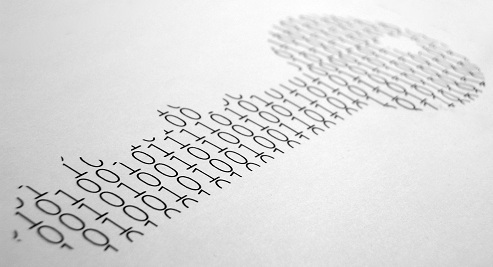
\includegraphics[scale=0.4] {./materials/cryptography.jpg} 
\end{center}
\end{frame}

%------------------------------------------------
\begin{frame}
\frametitle{Chiffrer - Les arguments contre}

\justifying{
\begin{block}{Personne ne le fait...}
FAUX. Sans le savoir, vous le faîtes tous les jours.
\\
Exemple 1: "le cadenas" quand on se connecte
\\  Exemple 2: La clef du Wifi.
\end{block}

\begin{block}{Je n'ai rien à cacher...}
FAUX. Qui accepterait que le facteur lise son courrier médical ?
\end{block}

\begin{block}{Le chiffrement, c'est pour les pédonazis de l'Internet...}
FAUX. Cas des journalistes/blogueurs dissidents qui dénoncent des dictatures...
\end{block}
}
\end{frame}

%------------------------------------------------
\begin{frame}
\frametitle{Chiffrer - Les arguments pour}

\begin{block}{Le chiffrement, ce n'est pas si compliqué}
Ce n'est pas plus compliqué que d'utiliser un "logiciel" ; i faut comprendre le principe et c'est du clickodrome.
\end{block}

\begin{block}{Protection et sécurité}
Mes données personnelles, sensibles sont protégées. Cf. PRISM, NSA...
\end{block}

\begin{block}{Confidentialité}
Seule la personne à qui est destiné le "message" est en mesure de le lire.
\end{block}

\end{frame}

%----------------------------------------------------------------------------------------
\begin{frame}
\frametitle{Edward Snowden}
\justifying{
Encryption works. Properly implemented strong crypto systems are one of the few things that you can rely on.
\begin{center}
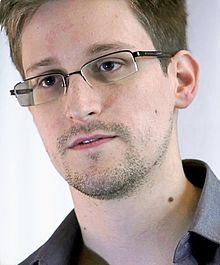
\includegraphics[scale=0.4] {./materials/snowden.jpg} 
\end{center}
Le chiffrement fonctionne. Correctement mis en œuvre, les systèmes cryptographiques forts sont l'une des rares choses sur lesquelles vous pouvez compter.
}
\end{frame}


%------------------------------------------------
\begin{frame}
\frametitle{Limites du chiffrement}
\begin{block}{Ce qui est chiffré aujourd'hui pourra être déchiffré demain}
\justifying{
Les ordinateurs de demain pourront permettre de décrypter les données chiffrées aujourd'hui.
}
\end{block}

\begin{block}{Si on perd la clef}
On n'a plus accès aux données.
\end{block}

\begin{block}{Métadonnées, graphe social}
\justifying{
\textbf{PGP ne protège pas contre l'analyse des métadonnée (serveurs de transit, adresses, headers, sujet).}
Ne pas oublier de nettoyer les métas-données des fichiers (tag EXIF des photos, documents de bureautiques avec le suivi des modifications).
DNS, cas du tracking Internet...}
\end{block}

\end{frame}

%----------------------------------------------------------------------------------------
\begin{frame}
\frametitle{Le chiffrement et la loi}
\justifying{
En France, la loi considère donc que l’utilisation de moyens de cryptologie est libre (LCEN article 30-1) et il n'y a donc, actuellement pas de limite à la taille de la clef de chiffrement que l'on peut utiliser.
\\~\\
En cas de perquisition,le refus de remise de la clef de chiffrement peut entraîner 3 ans d’emprisonnement ainsi que 45000\euro{} d’amende.
\\~\\
Cette peine est aggravée dans le cas où le chiffrement a été utilisé pour commettre un délit. 
\\~\\
Il est donc recommandé de donner la clef de déchiffrement, sauf dans le cas où les données déchiffrées entrainerait une procédure judiciaire dont la peine finale serait supérieure à celle de l'entrave à l'enquête judiciaire.
}
\end{frame}

